\subsection{Abast}

Com s'ha dit anteriorment, aquest projecte es centra en el desenvolupament d'una aplicació nativa per a dispositius iOS (iPhone, iPod i iPad) que consisteix en un client de la plataforma MAX. Aquesta aplicació ha d'incloure un conjunt de funcionalitats per tal de millorar la comunicació entre els usuaris d'una comunitat. Per fer-ho oferirà al usuari la possibilitat de crear activitats a en context concret i comunicar-se amb un sistema de missatgeria privada amb un altre usuari o un grup d'usuaris.

La gran dificultat que pot aparèixer durant el desenvolupament del projecte és tenir algun problema amb el MAX. Com que el MAX està desenvolupat per UPCnet, hi ha comunicació directe amb l'equip desenvolupador, per tal de poder solucionar qualsevol dubte o problema.

\begin{figure}[ht]
    \centering
    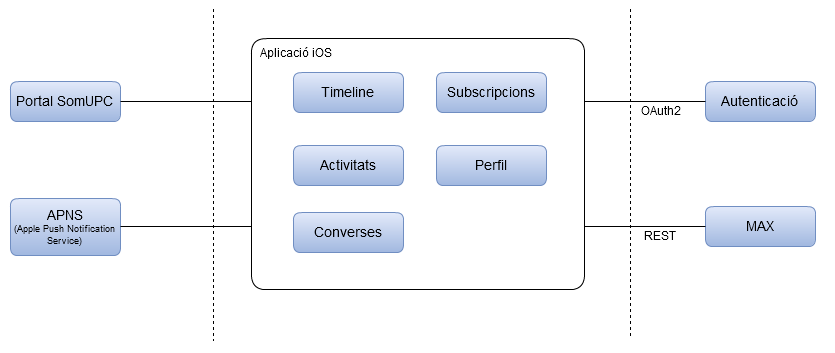
\includegraphics[scale=0.7]{Analisis/Abast/diagrama_context.png}
    \caption{Diagrama de context.}
    \label{fig:diagrama_context}
\end{figure}
\FloatBarrier

El projecte s'emmarca dintre del SomUPC, per tant és molt important delimitar les fronteres del sistema. El sistema a desenvolupar es tracta exclusivament de l'aplicació iOS, aquesta utilitzarà serveis externs, però aquests no formen part de l'abast. Al diagrama de context de la figura \ref{fig:diagrama_context} es poden veure clarament les barreres del projecte que delimiten l'abast.

L'aplicació utilitza el MAX com a font de l'activitat social, el portal SomUPC per a obtenir les fotografies dels usuaris, el APNS\footnote{Apple Push Notification Service} d'\textit{Apple} per a les notificacions \textit{push} i el servidor d'autenticació de la UPC per a l'autenticació dels usuaris.

